% !TEX TS-program = xelatex
% !TEX encoding = UTF-8 Unicode

% \documentclass[AutoFakeBold]{LZUThesis}
\documentclass[AutoFakeBold]{LZUThesis}

\begin{document}
%=====%
%
%封皮页填写内容
%
%=====%

% 标题样式 使用 \title{{}}; 使用时必须保证至少两个外侧括号
%  如: 短标题 \title{{第一行}},  
% 	      长标题 \title{{第一行}{第二行}}
%             超长标题\tiitle{{第一行}{...}{第N行}}

\title{{基于稀疏图码的离群值去除}}



% 标题样式 使用 \entitle{{}}; 使用时必须保证至少两个外侧括号
%  如: 短标题 \entitle{{First row}},  
% 	      长标题 \entitle{{First row}{ Second row}}
%             超长标题\entitle{{First row}{...}{ Next N row}}
% 注意:  英文标题多行时 需要在开头加个空格 防止摘要标题处英语单词粘连。
\entitle{{Outliers Removal Based on }{Sparse-Graph Codes}}

\author{庄启源}
\major{数学(基础理论班)}
\advisor{李朋}
\college{数学与统计学院}
\grade{2020级}



\maketitle

%==============================%
% ↓ ↓ ↓ 诚信说明页 授权说明书
%==============================%

% 1. 可以调整签字的宽度,现在是40
% 2. 去掉raisebox的相关注释(注意上下大括号对应),可以改变-5那个数字调整签名和横线的上下位置

% 你的签名,signature.pdf 改为你的签名文件名,
\mysignature{
    % \raisebox{-5pt}{
    
\includegraphics[width=50pt]{sign.pdf}
    % }
}
% 你手写的日期,signature.pdf 改为你的手写的日期文件名
\mytime{
    % \raisebox{-5pt}{
    
\includegraphics[width=80pt]{date.pdf}
    % }
}
% % 老师的手写签名,signature.pdf 改为老师的手写签名文件名
% \supervisorsignature{
%     % \raisebox{-5pt}{
%     
\includegraphics[width=40pt]{signature.pdf}
%     % }
% }
% % 老师手写的时间,signature.pdf 改为老师的手写的日期文件名
% \teachertime{
%     % \raisebox{-5pSt}{
%     
\includegraphics[width=40pt]{signature.pdf}
%     % }
% }
% % 老师手写的成绩
% \recommendedgrade{
%     % \raisebox{-5pt}{
%     
\includegraphics[width=40pt]{signature.pdf}
%     % }
% }

\makestatement

%==============================%
% ↑ ↑ ↑ 诚信说明页 授权说明书
%==============================%


%=====%
%论文(设计)成绩:注意2007的模板要求,成绩页在最后,2021要求成绩页在摘要前面
%=====%

% 下面这些注释掉可以去掉成绩、评语什么的
\supervisorcomment{ }


\committeecomment{ }

\finalgrade{ }
% 上面这些注释掉可以去掉成绩、评语什么的


\frontmatter



%中文摘要
\ZhAbstract{随着压缩感知理论研究的推进以及在工业界的大量应用,
众多解码方法被提出以更精确快速地重构稀疏度为$K$的高维稀疏信号$\mathbf{x} \in \mathbb{R}^{N}$。
为了更好地解决现实会遇到的信号恢复问题,我们研究在无噪声情形下当观测信号存在少量离群值时稀疏信号的精确恢复。
本文提出了一种离群值去除算法能够有效消除离群值在信号恢复中的巨大偏差影响。
在恢复过程中,我们应用稀疏图码相关理论,借由DFT矩阵和左正则二部图给出精心设计的测量矩阵。
由此实现的重构算法仅需对观测值进行几次简单的解码迭代即可精确恢复稀疏系数。
我们借助测量次数、恢复时间、精确恢复率等指标来评估信号重构算法。
特别地,本文展示了在无噪声情况下,我们的框架能够高效且稳定地恢复存在离群值的观测信号。
本文的所有源代码和数据公开在\href{https://github.com/waterEand/thesis_lzu}{\color{blue}\textit{https://github.com/waterEand/thesis\_lzu}}。
}
{压缩感知;离群值;稀疏信号恢复;稀疏图码}


%英文摘要-
\EnAbstract{With the advancement of research in compressed perception theory and its numerous applications in industry, 
numerous decoding methods have been proposed to fast reconstruct a high-dimensional $K$-sparse signal $\mathbf{x} \in \mathbb{R}^{N}$ accurately. 
In order to solve a signal recovery problem that may be encountered in reality more comprehensively, 
we study the exact recovery of sparse signals from the observations containing a few outliers without noise.
In this work, an outlier removal algorithm is proposed to effectively eliminate the influence of large deviations of outliers in signal recovery.
Through recovery, the measurement matrix is carefully designed through sparse-graph codes combined with the DFT matrix and the left regular bipartite graph.
A reconstruction algorithm is also implemented, 
by which the sparse coefficients can be recovered in a few iterations
by performing simple error decoding over the observations.
The signal reconstruction algorithm is evaluated by 
measuring times, time of recovery, rate of accurate recovery, etc.
Specifically, it is shown that in the absence of noise, 
our framework is able to efficiently recover observed signals in the presence of outliers steadily.
All source codes and data of our work are available at \href{https://github.com/waterEand/thesis_lzu}{\color{blue}\textit{https://github.com/waterEand/thesis\_lzu}}.
}
{Compressed sensing; Outliers; Sparse signal recovery; Sparse-graph codes
}

%生成目录
\tableofcontents
% 下面这个包含图表目录
% \customcontent


% % 部分同学需要专业术语注释表,* 表示不加入目录
% \chapter*{专业术语注释表}
% \begin{longtable}{lll}
%   \caption*{缩略词说明}\\
%   SS & Spread Spectrum & 扩展频谱 \\
%   PAPR & Peak to Average Power Ratio & 峰均比\\
%   DCSK & Differential Chaos Shift Keying &差分混移位键控\\
%   dasd & fdhfudw eqwrqw fasfasfs fewev wqfwefew &\tabincell{l}{太长了\\换行一下}\\
% \end{longtable}


%文章主体
\mainmatter

\chapter{\texorpdfstring{绪 \quad 论}{绪论}}

% !学校要求的规范,绪论是单独的,不是第一章,但是老师们都是让作为第一章,这里我把它放在了论文里,如果你要让在外面,只需要把上面的 \mainmatter 这一句话放在“绪论内容后面,正文第一章前面”即可,也就是 \chapter{latex部分用法简介} 这一句话上面


\section{问题介绍}

\subsection{压缩感知问题}

压缩感知(Compressed Sensing, CS)\cite{1614066}是一种利用信号稀疏性的信号采样理论。在有噪声情形,这一问题可被表达为:
对一个长度为$N$的稀疏信号$\mathbf{x}$,使用一个随机测量矩阵采样后得到一个长度为$M$的观测向量,再由该观测值估计初始信号。信号的压缩观测过程可表示为:
\begin{equation}
    \mathbf{y} = \mathbf{Ax} + \mathbf{w}
\end{equation}
这一过程被称为编码。其中$\mathbf{A}$是一个维数为$M \times N$的已知测量矩阵(观测矩阵),$\mathbf{w}$是一个可能的噪声向量,$\mathbf{y}$是观测值。

通常情况下,若$\mathbf{x}$没有特殊的结构或额外的信息,我们无法通过远少于该信号维度的测量次数(采样)来恢复$\mathbf{x}$。但是,如果信号是稀疏的或可压缩的,
即$\mathbf{x}$向量中只有$K$个非零元素($\mathbf{x}$的稀疏度为$K$)且$K << N$,那么我们就可以由极少次采样精确地恢复原信号。这一过程也被称为解码。
这种通过低维观测值重建高维信号的压缩感知方法被应用在各个领域中,
如医疗成像\cite{PMID:17969013}、天体物理学成像\cite{Wiaux_2009}、语音与图像处理\cite{elad2010sparse}等。

\subsection{次线性时间的支撑集恢复算法}

在压缩感知问题中,一个好的测量矩阵设计和高效的解码算法是极其重要的。为达到这一目的,我们可以从两个角度的问题入手:
要求能够保证信号精确恢复所需的观测次数$M$(即测量矩阵$\mathbf{A}$的行数)尽可能小;构建合适的测量矩阵$\mathbf{A}$使得恢复信号所需的时间复杂度尽可能小。

为同时达到这两个问题的最优,研究人员利用信号的稀疏性,提出了大量测量矩阵设计思路和信号重构算法来从低维观测值中恢复信号。
其中,大部分相关文献提出的稀疏信号恢复模型都主要基于$\ell_2 / \ell_1$范数或$\ell_1 / \ell_1$范数的近似误差指标,而基于支撑集恢复\cite{gilbert2010sparse}的工作就相对较少。
对于在不同观测情况下精确恢复信号支撑集的充要条件,学者们采取了
最优解码器\cite{861970, wainwright2007informationtheoretic}、
$\ell_1$极小\cite{10.1214/08-AOS653}、
贪心算法\cite{5895106}等策略进行研究。

其中,Wainwright\cite{wainwright2007informationtheoretic}提出,
在高斯噪声下,当测量矩阵的元素服从独立同分布(i.i.d.)的高斯分布时,
$O(K \log(N/K))$次测量(即$M = O(K \log(N/K)))$对于信号的支撑恢复是充分且必要的。
Bakshi、Jaggi\cite{7185441}等人提出的SHO-FA算法使有噪声情形下的信号恢复
仅需$O(K)$次测量且编码解码时间复杂度分别为$O(N)$和$O(K)$,这一结果达到了信息论中的阶次最优。
Li、Yin\cite{8733902}等人建立了一种新的压缩感知框架,能够在无噪声情况下,
用$2K$次测量精确地恢复任意稀疏度为$K$的信号,解码时间复杂度达到$O(K)$;
在有噪声情形,用$O(K \log(N/K))$次测量能达到同等效果,解码时间复杂度为$O(K \log(N/K))$。
并且文献\cite{8733902}提出的模型在$K$为次线性时,即存在$\delta \in (0,1)$使得$K = O(N^\delta)$,
测量次数和计算时间都与信号维数$N$成次线性关系,实现了概率保证下两者同时的阶次最优。

本文中我们将应用基于稀疏图码的算法\ref{8733902, Huaqiao}解决离群值去除后的问题,
使得总体测量次数和恢复时间都达到次线性的效果。

\subsection{基于稀疏图码的分治法}
\label{d_n_c}

我们通过通信系统中的稀疏图码来看待压缩感知问题,并用简单的“分治法”(分而治之)来处理稀疏信号。
如图\ref{fig_divide_conquer}的(a)所示,我们用不同的颜色表示稀疏向量$\mathbf{x}$中的不同元素,其中红色、绿色、蓝色方格表示非零元素,白色方格表示零元素。
在测量矩阵中,灰色方格表示随机生成的元素。相应生成的观测向量中每个元素则是红、绿、蓝颜色的混合。
\begin{figure}[H]
    \centering
    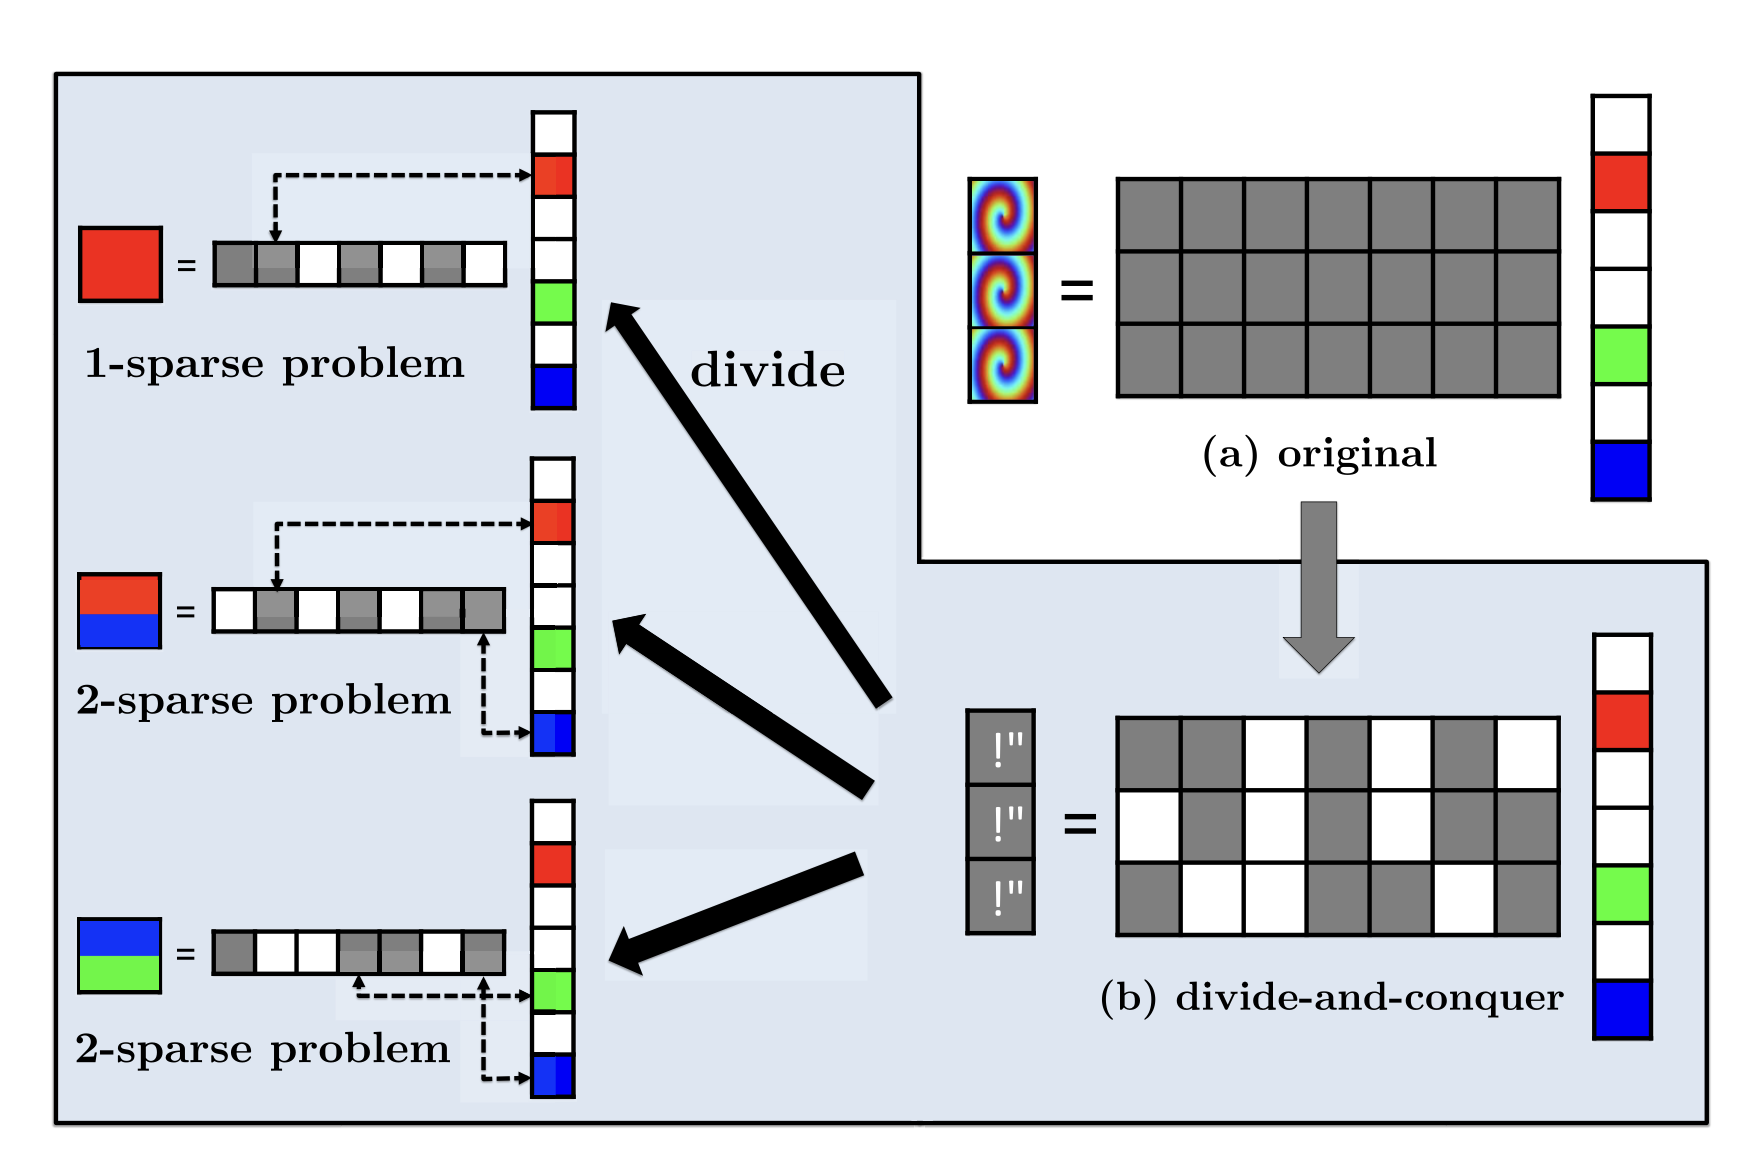
\includegraphics[width=0.7\textwidth]{figures/d_n_c.png}
    \caption{“分治法”的概念抽象图。
    子图(a)描绘一个稀疏度为3的恢复问题,其中测量矩阵着灰色,表示元素是随机生成的。
    由于不同颜色成分(红色、绿色、蓝色)随机混合,导致得到的观测结果呈现混合色。
    在子图(b)中,我们通过在每行中放置三个零元素来稀疏化测量矩阵,即图中的白色方格。
    由此产生的测量矩阵将稀疏度为3的恢复问题分解为多个稀疏度小于3的子问题。
    若子问题的观测值是单一颜色,我们可以立即恢复这一元素。
    在这一图中,第一个测量中的红色元素可以被立即恢复,之后再从第二个红蓝元素中把红色剥离,恢复蓝色,以此类推。}
    \label{fig_divide_conquer}
\end{figure}
在图\ref{fig_divide_conquer}的(b)中,我们用零元素(图中的空白格)来稀疏化测量矩阵的每一行。
这样设计的测量矩阵就导致了观测到的向量$\mathbf{y}$中包含的元素一部分是单一颜色,一部分是几种颜色的混合。
我们的设计理念就是把稀疏信号中的非零元分散到多个单一颜色的测量中(例如第一个测量中的红色),
然后从把这些单一颜色从混合颜色中剥离出来(例如第二个测量中的红蓝混合和第三个测量中的蓝绿混合),
如此迭代逐步解码其他颜色的未知元素,这也就是“分治”的过程。
稀疏图码在这里的作用本质上是将一般的稀疏信号重构问题分解为多个可以轻松解决的子问题,
最后再把这些子问题的结果融合以恢复所有非零元素。
这样的设计兼具了稀疏图编码在测量成本(容量逼近)和计算复杂性(基于快速剥离的解码)方面的特性,
从而使稀疏测量矩阵达到了低测量次数和低计算成本的效果。


\section{研究意义与目的}

考虑到压缩感知常被应用在图像采样的任务中,且采样过程可能会出现探头损坏,导致得到的观测值会出现离群值(Outliers)的情况,
本文研究在无噪声情形下,观测值中存在部分离群值的稀疏信号的解码恢复。该观测过程可表示为:
\begin{equation}
    \mathbf{y} = \mathbf{Ax} + \mathbf{f}
\end{equation}
其中$\mathbf{f}$是一个维数为$M$的离群向量,$\mathbf{f}$中的非零元素(离群值)个数$T$远小于$M$,
满足$\left | \mathrm{supp} (\mathbf{f}) \right | = T = \eta M \ (0 \leq \eta < \frac{1}{2})$,
且这些离群值的分布方差显著大于$\mathbf{x}$中的非零元素。
我们的目标是尽可能去除$\mathbf{y}$的非零元素中的所有离群值,并着眼于精确地恢复稀疏度为$K$长度为$N$的信号的支撑集(稀疏体系)以及相对应的稀疏系数。

支撑集恢复结果的一个经典误差评价指标是信号支撑集无法被精确恢复的概率,
即$\mathrm{Pr}(\mathrm{supp}(\hat{\mathbf{x}}) \neq \mathrm{supp}(\mathbf{x}))$,
其中$\mathrm{supp}(\mathbf{x}) \coloneq \{k:\ x[k] \neq 0,\ 0 \leq k \leq N-1\}$。
也就是说,对于任意给定的稀疏度为$K$长度为$N$的信号$\mathbf{x}$,我们设计一个测量矩阵$\mathbf{A}$,并计算出一个估计向量$\hat{\mathbf{x}}$,
并且希望这一个估计的支撑集与原信号$\mathbf{x}$的支撑集完全匹配的概率接近于$1$。

同时,我们也要恢复$\mathbf{x}$中的稀疏系数,也就是要恢复信号中非零元的精确值。
对于这一恢复,我们目标得到较强的$\ell_{\infty}$和$\ell_{1}$范数保证。 
这里,我们采取非均匀保证\cite{gilbert2010sparse},也就是采用单个测量矩阵来恢复特定的单个稀疏信号。
相对地,均匀保证是指仅用一个测量矩阵恢复一次生成的所有稀疏信号(多个),这里不做讨论。

兼顾以上两个要求,我们制定评价指标为信号被精确恢复的概率,具体定义将在第\ref{result}章给出。
我们的目的就是提高这一概率,并与其他经典模型比较。

\section{本文的贡献}

在本文中,我们基于稀疏图码把稀疏度为$K$的信号恢复问题转化为求解多个稀疏度为$1$维数为$N$的信号恢复问题,
并进一步探讨存在离群值情况下的问题,提出一种基于分位数的离群值去除算法。
通过最后的数值实验讨论我们算法的性质,
并与传统的PLAD算法\cite{doi:10.1137/090777761, WANG2013135}对比
来证明其在时间和精确程度上的有效性。
% 且解码过程中每个元素的测量次数及其恢复时间的数量级都达到$O(1)$。
% 在离群值去除后,由逐步剥离算法保证信号的恢复。我们选择离散傅立叶变换(\eqrm{DFT})矩阵的前两行作为在稀疏图码作用前的检测矩阵。
% 在解码过程中,我们通过这一检测矩阵计算信号非零元的位置,然后基于稀疏度为$1$的性质精确恢复该系数。
% 每个元素的测量次数及其恢复时间的数量级都为$O(1)$。由于信号中共有$K$个稀疏系数需要去估计,总共的测量次数和恢复时间复杂度与$O(K)$成线性关系。

\chapter{测量矩阵的设计}

在本章中,我们将从章节\ref{d_n_c}描述的理念出发,借助简单例子介绍测量矩阵$\mathbf{A}$的具体设计方法。

我们考虑一个长度$N=16$,稀疏度$K=4$的稀疏信号$\mathbf{x}$。其中包含有非零元素$x[1] = 1$,$x[4] = 4$,$x[8] = 2$,$x[13] = 7$。
接下来我们构建一个左节点数为16,右节点数为9的二部图。如图\ref{fig_bip_graph}所示,这个图有以下性质:

\begin{itemize}
    \item 每个左节点$x[k]$都连接至少一个右节点。
    \item 每个右节点$y_r$的值是与其相连接的的左节点值的和。
\end{itemize}

\begin{figure}[H]
    \centering
    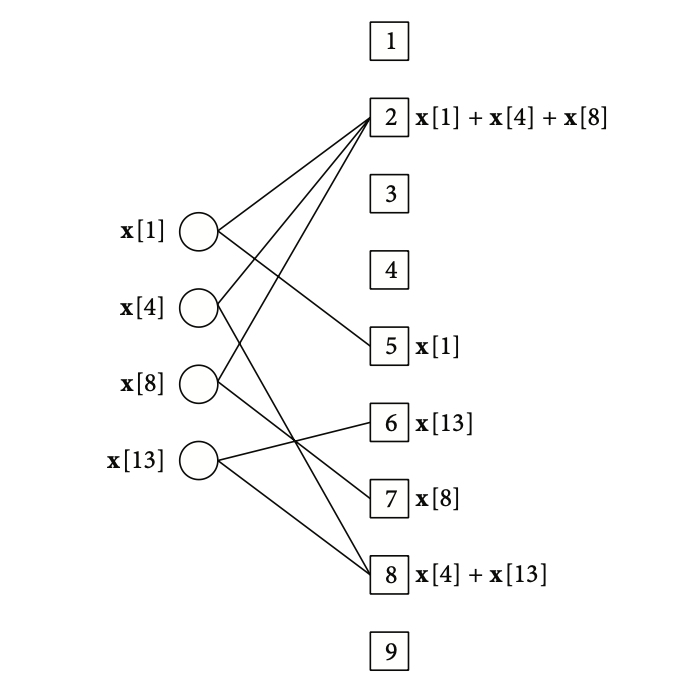
\includegraphics[width=0.55\textwidth]{figures/bip_g.png}
    \caption{稀疏测量二部图}
    \label{fig_bip_graph}
\end{figure}

这样就形成了对于长度为16的稀疏信号$\mathbf{x}$(左节点)的9次测量:
\begin{equation*}
    \begin{aligned}
        y_1 &= y_3 = y_4 = y_9 = 0, \\
        y_2 &= x[1] + x[4] + x[8], \\
        y_5 &= x[1], \\
        y_6 &= x[13], \\
        y_7 &= x[8], \\
        y_8 &= x[4] + x[13].
    \end{aligned}
\end{equation*}
根据稀疏测量二部图的连通性,我们将与右节点分为以下三种类型:
\begin{enumerate}
    \item \textbf{零节点}:若一个右节点不包含任何非零元素,则称其为零节点,如图\ref{fig_bip_graph}的$y_1$。
    \item \textbf{单节点}:若一个右节点仅包含一个非零元素,则称其为单节点,如图\ref{fig_bip_graph}的$y_5$。
    \item \textbf{多节点}:若一个右节点包含一个以上的非零元素,则称其为多节点,如图\ref{fig_bip_graph}的$y_2$。
\end{enumerate}
其实单节点就是章节\ref{d_n_c}描述的单一颜色的元素,多节点就是混合颜色。
我们从单节点入手进行逐步剥离解码,具体算法将在第\ref{solu}章介绍。

为了判断观测向量中的元素(右节点)属于哪种节点,
我们给每个左节点不同的2维向量加权,于是每个右节点可被表示为几个二维向量之和。
为此我们设计一个列数与信号$\mathbf{x}$长度相同的检测矩阵$\mathbf{S}$:
\begin{equation}
    \mathbf{S}=
    \left[
        \begin{array}{ccccccc}
            1 & 1 & 1  & 1 & 1 & \dots & 1 \\
            1 & W & W^2 & W^3 & W^4 & \dots & W^{15}
        \end{array}
        \right],
    \label{S}
\end{equation}
其中$W = e^{i \frac{2\pi}{N}}$是一个$N$次单位根,这里的例子中$N = 16$。
$\mathbf{S}$是一个$16 \times 16$的DFT矩阵的前两行,通过$\mathbf{S}$检测节点的具体算法将在章节\ref{solu}介绍。

除此之外,我们还需要定义一个编码矩阵$\mathbf{H}$来表示二部图左右节点的连接,
$\mathbf{H}$在这个例子中是一个$9 \times 16$的由0和1组成的邻接矩阵。

为了将$\mathbf{H}$和$\mathbf{S}$结合在一起形成完整的测量矩阵$\mathbf{A}$,
下面我们介绍\textbf{行张量算子} $\boxtimes$(row-tensor operator)的定义。一般情况下,
检测矩阵$\mathbf{S} = \left[\mathbf{s}_0, \cdots, \mathbf{s}_{N-1}\right] \in \mathbb{C}^{M_2 \times N}$,
邻接矩阵$\mathbf{H} = \left[\mathbf{h}_0, \cdots, \mathbf{h}_{N-1}\right] \in \mathbb{C}^{M_1 \times N}$。
行张量运算$\mathbf{H} \boxtimes \mathbf{S}$本质上就是
将矩阵$\mathbf{H}$的每一行通过与矩阵$\mathbf{S}$中每个相应的列进行逐个元素的增广。
我们得到的行张量积是一个维数为$M_1 M_2 \times N$的矩阵:
\begin{equation*}
    \mathbf{H} \boxtimes \mathbf{S} = \left[\mathbf{h}_0 \otimes \mathbf{s}_0 , \cdots , \mathbf{h}_{N-1} \otimes \mathbf{s}_{N-1} \right],
\end{equation*}
其中$\otimes$是一个标准的克罗内克积(Kronecker product)。下面我们举一个简单例子来具象化这一过程。
我们设定
\begin{equation}
    \mathbf{H} = 
    \left[
        \begin{array}{ccccccc}
            1 & 1 & 0 & 1 & 0 & 1 & 0 \\
            0 & 1 & 0 & 1 & 0 & 0 & 1 \\
            1 & 0 & 0 & 1 & 1 & 0 & 1
        \end{array}
    \right], 
\end{equation}
\begin{equation}
    \mathbf{S} = 
    \left[
        \begin{array}{ccccccc}
            1 & 1 & 1  & 1 & 1 & 1 & 1 \\
            1 & W & W^2 & W^3 & W^4 & W^5 & W^6
        \end{array}
    \right], 
\end{equation}
这里$W = e^{i \frac{2\pi}{7}}$。那么我们就可以计算出行张量积:
\begin{equation}
    \mathbf{H} \boxtimes \mathbf{S} = 
    \left[
        \begin{array}{ccccccc}
            1 & 1 & 0 & 1 & 0 & 1 & 0\\
            1 & W & 0 & W^3 & 0 & W^5 & 0\\
            0 & 1 & 0 & 1 & 0 & 0 & 1 \\
            0 & W & 0 & W^3 & 0 & 0 & W^6 \\
            1 & 0 & 0 & 1 & 1 & 0 & 1\\
            1 & 0 & 0 & W^3 & W^4 & 0 & W^6
        \end{array}
    \right].
\end{equation}
在本例中,$\mathbf{H}$有三行,分别与$\mathbf{H} \boxtimes \mathbf{S}$的前两行,中间两行,后两行对应。

用这种方式,我们可以生成一个测量矩阵$\mathbf{A} = \mathbf{H} \boxtimes \mathbf{S} \in \mathbb{C}^{M_1 M_2 \times N}$,
这样得到观测值$\mathbf{y} \in \mathbb{C}^{M_1 M_2}$。
\begin{definition}[测量矩阵]
    设$M = RP$且$P, R \in \mathbb{N}^*$。
    给定一个$R \times N$的编码矩阵$\mathbf{H}$和一个$P \times N$的检测矩阵$\mathbf{S}$,
    那么$M \times N$的测量矩阵$\mathbf{A}$就可被定义为:
    \begin{equation}
        \mathbf{A} = \mathbf{H} \boxtimes \mathbf{S},
    \end{equation}
    其中$\boxtimes$是行张量算子,并且编码矩阵和检测矩阵满足下述条件:
    \begin{itemize}
        \item 编码矩阵$\mathbf{H} = [H_{r, n}]_{R \times N}$是一个关于二部图$\mathcal{G}$的邻接矩阵。
        图$\mathcal{G}$包含$N$个左节点$V_1 \coloneq [N]$和$R$个右节点$V_2 \coloneq [R]$,边的集合为$\mathcal{E} \coloneq V_1 \times V_2$。
        \item 检测矩阵$\mathbf{S} \coloneq \left[\mathbf{s}_0, \cdots, \mathbf{s}_{N-1}\right]$是一个$N \times N$的DFT矩阵的前$P$行。
    \end{itemize}
\end{definition}

\chapter{求解算法}

本章将介绍在测量矩阵设计完毕的基础上,离群值去除以及信号恢复问题的具体算法求解。

\section{节点类型检测}

我们继续借用图\ref{fig_bip_graph}的例子来模拟算法。由公式$\ref{S}$可知,
我们可以通过$\mathbf{S}$把每个右节点都记为一个二维向量$\mathbf{y}_r = [y_r[0], y_r[1]]^T$,
我们称每个这样的向量为一个\textbf{测量对}(measurement bin)。
在上述例子中,
右节点1,2,5的测量就可以被记为:

\begin{equation*}
    \begin{aligned}
        \mathbf{y}_1 &= \mathbf{0}, \\
        \mathbf{y}_2 &= x[1] \times 
        \left[
            \begin{array}{c}
                1 \\ W
            \end{array}
        \right] + x[4] \times 
        \left[
            \begin{array}{c}
                1 \\ W^5
            \end{array}
        \right] + x[8] \times
        \left[
            \begin{array}{c}
                1 \\ W^8
            \end{array}
        \right], \\
        \mathbf{y}_5 &= x[1] \times
        \left[
            \begin{array}{c}
                1 \\ W
            \end{array}
        \right]. 
    \end{aligned}
\end{equation*}

于是通过对测量对的检测,我们能够有效地确定右节点是零节点、单节点还是多节点。
我们由右节点1,2,5的例子介绍节点检测的方法:

\begin{enumerate}
    \item \textbf{零节点对}:参考右节点1。若测量对是一个全0向量,即$\mathbf{y}_r = \mathbf{0}$,则该节点为零节点。
    \item \textbf{单节点对}:参考右节点5。这个测量对满足比值检测:
        \begin{equation*}
            \hat{k} = \frac{\angle y_5[1] / y_5[0]}{2 \pi / 16} = 1, 
        \end{equation*}
        其中$\hat k$为整数,则该节点就是单节点。于是
        \begin{equation*}
            \hat x [\hat k] = y_5 [0]. 
        \end{equation*}
        我们也就从中顺利恢复了信号$\mathbf{x}$中的非零元素$x_1$。另一种检测方法是,
        这样的单节点对的两个元素的模一定相等,即$|y_3[0]| = |y_3[1]|$。
        因为$W$是单位根,$|W^r| = 1$。
    \item \textbf{多节点对}:参考右节点2。对这个测量对进行比值检测:
        \begin{equation*}
            \hat k = \frac{\angle y_2[1] / y_2[0]}{2 \pi / 16} = 4.85995. 
        \end{equation*}
        并且两个元素的模并不相等,$|y_2[1]| \neq |y_2[0]|$。
        在这种比值检测的结果$\hat k$不为非零整数或两个元素不同模的情况下,该节点为多节点。
\end{enumerate}
综上,要判断任意非零节点对$y_r$的类型,我们只需计算
\begin{equation}
    \label{k}
    \hat k = \frac{\angle y_r[1] / y_r[0]}{2 \pi / N},
\end{equation},
当$\hat k$为整数,则该节点是单节点;反之则为多节点。

\section{离群值去除}
\label{removal}
离群值(outliers),也被称为异常值,是指与其他观察结果显著不同的数据点。
存在离群值情况下,压缩观测过程可被描述为$\mathbf{y} = \mathbf{Ax} + \mathbf{f}$。
其中$\mathbf{f} = [f_1, f_2, \dots, f_M]^T$,且
$\left | \mathrm{supp} (\mathbf{f}) \right | = T = \eta M \ (0 \leq \eta < \frac{1}{2})$。
我们设初始稀疏度为$K$的稀疏信号$\mathbf{x}$中的非零元素服从均值为0,标准差为1的高斯分布,即$x_i \sim N(0, 1), i \in [N]$。
稀疏度为$\eta$的离群向量$\mathbf{f}$中的非零元素满足$f_j \sim N(0, 100), j \in [M]$。

从中我们可以显然得到:$\mathbf{f}$中大部分非零元素的绝对值远大于$\mathbf{x}$中元素的绝对值。
为了尽可能剔除这些离群值,又考虑到$\mathbf{y}$的稀疏性,
我们可以尝试取$\mathbf{y}$的非零元素绝对值的某个分位数$\theta_p$($p$是一个分位数算子,常取0.5、0.75),
并且设定一个倍率$\alpha$得到一个分界数$\alpha \cdot \theta_p$,
抹去$\mathbf{y}$的非零元素中所有绝对值大于$\alpha \cdot \theta_p$的数的集合。
这里“抹去”的定义是将这些非零元素设为0,也就是这些元素不参与信号重构的过程。

用数学语言描述,我们把$\mathbf{y}$的有效非零元素限制在一个指标集
$S = \{s: |y_s| < \alpha \theta_p (\{|y_j| : j \in \mathrm{supp} (\mathbf{y})\})\}$上,
其他指标的对应元素全部设为0。
例如,当$\alpha = 1, p = \frac{1}{2}$时,我们就抹去所有绝对值大于非零元素绝对值中位数的数。
这样就理论上去除了全部绝对值过大的离群值,
接下来对被限制的$\mathbf{y}$应用信号重构算法即可。

由于离群向量$\mathbf{f}$的稀疏度$T$是未知的,我们无法简单地抹去绝对值最大的前$T$个元素,因此采取上述设置比例或分界数的方式。
我们又知道$\mathbf{y}$和$\mathbf{f}$都是稀疏的,所以$\mathbf{y}$和$\mathbf{f}$的支撑集大概率不会存在元素位置重合的情况,
不会抹去需要参与信号恢复的非离群值。因此,这样直接设为0的方式是合理且可取的。算法伪代码如下:

\begin{algorithm}[H]
    \caption{离群值去除算法\label{Alg:outliers_removal}}
    \begin{algorithmic}[1]
        \State \textbf{输入}:一个观测值 $\mathbf{y} \in \mathbb{C}^{2R}$(测量对形式),常数$\alpha$。
        \State 首先计算得到$\mathbf{y}$的非零元素模的中位数$med = \mathbf{Median}(\{|\mathbf{y}_j[0]|: \mathbf{y}_j[0] \neq 0, \mathbf{y}_j \in \mathbf{y}\})$;
        \For{$r = 1$ to $R$}
            \If{$|\mathbf{y}_r [0]| > \alpha \cdot med$}
                \State 将$\mathbf{y}_r$抹去为$\mathbf{0}$向量;
            \EndIf
        \EndFor
    \end{algorithmic}
\end{algorithm}

\section{信号恢复}
\label{solu}

本节将聚焦于离群值已去除的信号恢复。经过上述铺垫,我们按照以下步骤解码即可(参考\ref{d_n_c}):

\begin{enumerate}[1) ]
    \item 选取二部图中所有使得右节点度数为1的边(找到所有单节点)
    \item \label{step2}去除(剥离)所有这些边以及与之对应的左右节点对。
    \item \label{step3}去除(剥离)步骤\ref{step2}中剥离的左节点的其他未被剥离的边。
    \item 找到步骤\ref{step3}中去除的左节点连接的所有右节点,将这些左节点的值从右节点的值中减去。
\end{enumerate}
伪代码如下:

\begin{algorithm}[H]
    \caption{剥离解码器\label{Alg:peeling_decoder}}
    \begin{algorithmic}[1]
        \State \textbf{输入}:一个观测值 $ \mathbf{y} \in \mathbb{C}^{2R} $ (测量对形式),待恢复信号$\mathbf{\hat x} = \mathbf{0}$。
        \For{$i = 1,2, \ldots $ 直到$\mathbf{y}^{(i)} = \mathbf{0}$或找不到单节点}
            \For{$r = 1$ to $R$}
            \State 由公式$\ref{k}$计算$\hat k$,判断$\mathbf{y}_r^{(i)}$是否为单节点对;
                \If{$\mathbf{y}_r^{(i)}$是单节点}
                    \State $\mathbf{\hat x}[\hat k] = \mathbf{y}_r^{(i)}[0]$;
                    \For{$r^{\prime} = 1$ to $R$}
                        \State 找到连接左节点$\hat k$的右节点$r^{\prime}$;
                        \State 剥离过程$\mathbf{y}_{r^{\prime}}^{(i+1)} = \mathbf{y}_{r^{\prime}}^{(i)} - \hat{x}[\hat k]\mathbf{s}_{\hat k}$,
                        这里$\mathbf{s}_{\hat k}$是检测矩阵$\mathbf{S}$的第$\hat k$列;
                    \EndFor
                \Else
                    \State 继续下一个节点对$\mathbf{y}_{r+1}^{(i)}$。
                \EndIf
            \EndFor
        \EndFor
    \end{algorithmic}
\end{algorithm}

\chapter{数值实验结果}
\label{result}

本章我们对无噪声条件下存在离群值的信号恢复问题进行数值模拟,从实验角度出发论证理论内容。
在本章的实验中,我们通过上一章描述的剥离算法对不同情况的离群值问题进行求解。
先验证算法在不同情形下的高效性,再与其他算法做比较来证明我们算法的优越性,
之后比较观测离群值去除算法参数不同时的恢复效果。

我们将实验的参数统一设置为:$N = 200$;初始稀疏信号$\mathbf{x} \in \mathbb{R}^N$且其中元素服从$x_i \sim N(0,1)$;
邻接矩阵$\mathbf{H} \in \{0, 1\}^{M \times N}$;检测矩阵$\mathbf{S}$为$N \times N$的DFT矩阵前两行;
离群向量$\mathbf{f}$中的非零元素服从$f_j \sim N(0,100)$。
本文中数值实验均由Python3.11.3实现,在macOS Sonoma 14.2.1操作系统下,
用一块Apple M2 Pro(CPU)芯片完成运行。

为了衡量信号恢复的误差,我们定义评价指标\textbf{精确恢复率}为多次重复实验中
恢复结果误差$err < thr\_err$的次数与总实验次数的比值。
这里$err = \frac{||x- \hat x||_2}{||x||_2}$,其中$x$是初始信号,$\hat x$为恢复结果;
$thr\_err$是界定一次信号恢复是否成功的阈值。
在实验的大多数情况下我们取$thr\_err = 10^{-7}$;
而由于我们将对比的传统算法(PLAD算法)无法达到这样的准确度,我们在对比实验中取$thr\_err = 10^{-2}$。
当$err < thr\_err$,我们称信号被精确恢复一次。


\section{信号恢复效率}

在本节中我们先通过几个实验,用信号精确恢复所需测量次数和恢复用时两个角度来评估我们算法的恢复精确度及高效性。

\subsection{不同测量次数下的恢复效率}
在第一个实验中,测量值数目$M$作为自变量。
我们设定$\mathbf{x}$的稀疏度为2;
$\mathbf{H}$为每列有且仅有三个1的矩阵,即表示正则度为3的左正则二部图;
离群值比例$\eta$为0.01;
离群值去除算法中$\alpha = 2, p = \frac{1}{2}$;
重复实验次数为500次。结果如下:

\begin{table}[H]
    \centering
    \caption{不同测量次数下信号恢复时间及恢复效果}
    \begin{tabular}{ccccccc} % 控制表格的格式,可以是l,c,r
        \toprule
        测量值数目$M$ & 10  & 20  & 40  & 80 & 100 & 120 \\
        \toprule
        精确恢复率 & 70.0\% & 84.5\% & 90.5\%  & 92.5\% & 95.5\% & 95.0\% \\
        \midrule
        平均用时(毫秒) & 48.55 & 79.25 & 89.70 & 95.40 & 115.25 & 126.50 \\
        \bottomrule
    \end{tabular}
    \label{effeciency}
\end{table}

由表\ref{effeciency}可知仅需100次的测量就可95\%精确地恢复存在一个离群值的稀疏度为2的信号$\mathbf{x} \in \mathbb{R}^{200}$,
且在500次随机实验中每次恢复所需时间仅0.115秒左右。

\subsection{不同信号稀疏度下的恢复效率}

在第二个实验中,信号稀疏度$K$作为自变量。
我们设定$M = 100$;
离群值去除算法中$\alpha = 2, p = \frac{3}{4}$;
其他与上一个实验相同。
结果如下:

\begin{table}[H]
    \centering
    \caption{不同信号稀疏度下信号精确恢复的概率}
    \begin{tabular}{cccccc} % 控制表格的格式,可以是l,c,r
        \toprule
        稀疏度$K$ & 1  & 2  & 3  & 4 & 5\\
        \toprule
        精确恢复率 & 98.0\% & 95.5\% & 92.2\%  & 91.7\% & 88.8\%\\
        \midrule
        平均用时(毫秒) & 124.0 & 129.0 & 129.6 &  125.4 & 130.4\\
        \bottomrule
    \end{tabular}
    \label{diff_sprs}
\end{table}

在表\ref{diff_sprs}我们可以看到信号稀疏度越小,恢复越精确;
平均每次信号恢复时间为$0.124 \sim 0.130$秒,
总体上稀疏度$K$越大恢复所需时间越长。

\subsection{不同离群值比例下的数值效果}

在离群向量$\mathbf{f}$中$\left | \mathrm{supp} (\mathbf{f}) \right | = \eta M$。
显然,随着离群值比例$\eta$的增大,信号恢复的难度也越来越大。
本次实验中我们探索离群值比例变化给恢复效果带来的变化程度,
设定信号稀疏度$K = 2$,离群值去除算法中$\alpha = 1, p = \frac{1}{2}$,其他与上一小节相同。
由于本次实验中恢复时间基本相同(最大差值不超过5毫秒),我们不再列举平均每次恢复用时。
实验结果如下:

\begin{table}[H]
    \centering
    \caption{不同离群值比例下信号精确恢复的概率}
    \begin{tabular}{cccccc} % 控制表格的格式,可以是l,c,r
        \toprule
        离群值比例$\eta$ & 0.01  & 0.02  & 0.03  & 0.04 & 0.05\\
        \toprule
        精确恢复率 & 91.2\% & 90.4\% & 88.0\%  & 85.6\% & 82.8\%\\
        \bottomrule
    \end{tabular}
    \label{diff_eta}
\end{table}

这里信号恢复效果较差,是因为离群值比例变化下,中位数倍率并没有变化。
若对每一个$\eta$下的中位数倍率$\alpha$进行微调,我们能得到每个精确恢复率都高于$90\%$的效果。
由表\ref{diff_eta}可见当离群值比例$\eta$大于0.02时,算法恢复效果显著降低,且精确恢复率下降速度极快。

\section{离群值去除算法的参数大小对数值效果的影响}
\label{diff_params}
本节实验中我们探究离群值去除算法的参数大小(包括$\alpha$和$p$)对恢复效果的影响。
在直觉上,离群值比例越高,倍率$\alpha$就要更小(或$p$更小)来保证去除所有离群值。
这里我们选取$\mathbf{x}$的稀疏度$K = 2$,分位数$\theta_p$中的分位数算子$p = 0.5$,$\mathbf{H}$和评价指标均与上述实验相同。
这里只讨论倍率$\alpha$的影响,是因为由章节\ref{removal}可知,
离群值去除的分界数是$\alpha \theta_p$,
因此模拟的数值实验中$\alpha$的变化和$p$的变化是等价的。
我们通过离群值比例$\eta$不同的实验,对精确恢复率随倍率$\alpha$的变化进行展示。
结果如下图:
\begin{figure}[H]
    \centering
    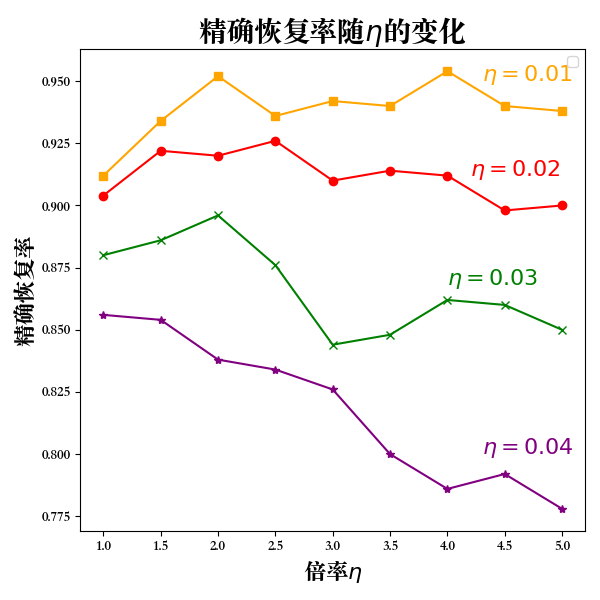
\includegraphics[width=0.7\textwidth]{figures/diff_eta.png}
    \caption{不同离群值比例下的恢复效果随算法参数变化展示。
        图中横坐标表示不同的倍率$\alpha$,纵坐标表示精确恢复率,
        四条曲线分别表示离群值比例取$1\%, 2\%, 3\%, 4\%$的情形。
        }
    \label{fig_diff_alg}
\end{figure}

由图\ref{fig_diff_alg}可知,随离群值比例增大,
我们需要调小倍率$\alpha$(或调小$p$)来保证较好的恢复效果。
当离群值比例超过0.03时,精确恢复概率无法达到期望。

因此,当我们在解决离群值极少的任务时,可以选择较大的倍率$\alpha$或分位数算子$p$;
而在大多数情况下,选择小的倍率显然是更加稳定的。

\section{与其他信号恢复算法的比较}

为了说明我们提出的算法的存在意义与优越性,我们将算法与其他传统算法对比,
比较同等情况下两者的精确恢复率和恢复所需时间。
我们选择对比算法为$\ell_1$-PLAD算法(Penalized Least Absolute Deviation),
因为这是信号恢复领域非常经典且能够解决离群值问题的算法。
其他算法如LASSO、DS、RPDS等算法都无法去除偏差较大的离群值,故不做比较。
$\ell_1$-PLAD算法的原理可以简单描述为:
\begin{equation}
    \min_{\mathbf{x} \in \mathbb{R}^N}{||\mathbf{y} - \mathbf{Ax}||_1 + \lambda ||\mathbf{x}||_1}
\end{equation}
其中$\mathbf{A}$是一个$M \times N$的高斯测量矩阵。

在本节实验中,我们设置$\mathbf{x}$的稀疏度为3,$M = 100$,离群值比例取0.02和0.03,编码矩阵$H$和重复实验次数与上一节相同。
我们的算法中$\alpha = 2, p = \frac{1}{2}$;$\ell_1$-PLAD算法中迭代次数为2000次,
$\lambda$作为自变量,且$\lambda \in [0.006, 0.009$]
(经检验,$\lambda$超出这一区间的PLAD算法精确恢复率无法高于50\%)。
另外与本文其他实验不同的是,这里$thr\_err = 10^{-2}$,
因为PLAD算法无法达到我们的算法能达到的$err < 10^{-7}$的精度。
实验结果如下(下表中间部分的数值为精确恢复率):

\begin{table}[H]
    \centering
    \caption{我们的离群值去除算法与PLAD算法的对比}
    \begin{tabular}{cccccc} % 控制表格的格式,可以是l,c,r
        \toprule
        应用算法 & 我们的算法  & \eqrm{PLAD_{\lambda = 0.006}}  & \eqrm{PLAD_{\lambda = 0.007}}  & \eqrm{PLAD_{\lambda = 0.008}} & \eqrm{PLAD_{\lambda = 0.009}}\\
        \toprule
        $\eta = 0.02$ & 92.0\% & 78.2\% & 94.6\% & 91.2\%  & 79.8\%\\
        \midrule
        $\eta = 0.03$ & 89.8\% & 47.8\% & 66.4\% & 92.2\%  & 92.0\%\\
        \toprule
        平均用时(毫秒) & 129.0 & 1729.9 & 1268.3 & 1692.2 &  2374.5\\
        \bottomrule
    \end{tabular}
    \label{diff_algs}
\end{table}

由此可见PLAD算法的平均恢复所需用时远高于本文提出的算法,
在最好情况下也有10倍的差距,因此PLAD显然无法用于实时的存在离群值的信号恢复任务。

另外,PLAD算法虽然在一定条件下能达到更加精确的结果,但是总体恢复效果受参数$\lambda$大小的影响极严重。
例如,由表\ref{diff_algs},倘若我们取$\lambda=0.007$,这一算法在离群值只占0.02比例时恢复效果极好,
而一旦离群值比例轻微变化,上升到0.03,精确恢复率就急剧下降到小于70\%。
而由\ref{diff_params}节可知,我们提出的算法受参数大小影响并不严重。
因此,我们的算法相较PLAD更能胜任多情形下(更一般)的快速信号恢复任务。

\chapter{总结与展望}

本文研究了存在少量离群值时稀疏信号的恢复。我们先介绍了用二部图生成邻接矩阵,
再提出了一种离群值去除方式,并与前人提出的基于稀疏图码的次线性时间解码算法结合,
通过先去除再恢复的两阶段法达到精确恢复信号的目的。
我们通过数值实验论证了算法的有效性,
通过与传统的PLAD算法比较展示我们方法的性能:
恢复仅需极短的CPU时间,
且对不同的情况更具一般性,也不会因算法参数变化产生极大波动。

我们也可以进一步研究拓展到稀疏低秩矩阵恢复的情形,
与文献\cite{10120641}改进的算法结合,也可能有较好的效果。
另外,文中没有讨论编码矩阵$\mathbf{H}$的具体设计策略,
我们选择的是左正则二部图生成的二元稀疏矩阵,
而其他满足RIP条件的矩阵可能会有更好的效果。


% \input{test.tex}


%论文后部
\backmatter


%=======%
%引入参考文献文件
%=======%
\bibdatabase{bib/database}%bib文件名称 仅修改bib/ 后部分
\printbib
% \nocite{*} %显示数据库中有的,但是正文没有引用的文献



\Appendix

% python代码
\section{主算法代码}

主程序文件
% peeling\_decoder\_vector.py

\begin{lstlisting}[language = python]
    # peeling_decoder_vector.py

    import random
    import time
    import numpy as np
    import scipy as sp
    import cmath
    from signal_vectors import signal_vec, outliers
    from scipy.sparse import csr_matrix
    from numpy import linalg as LA

    # parameters to be modified
    n = 200 # N
    R = 100 # M
    k = 2 # sparsity of x
    density_H = 3
    num_outliers = 1
    med_times = 2 
    percent = 50 # p
    var_outliers = 100 # variance of outliers
    thr_err = 1e-7
    num_epoch = 500
    
    def input_vector(n, k):
        x = signal_vec(n, k)
        return np.squeeze(x)
    
    def H_measure(row, col, k):
        res = np.zeros((row, col))
        for i in range(col):
            rvs = sp.stats.bernoulli(1).rvs
            S = sp.sparse.random(row, 1, density=k/row, data_rvs=rvs)
            res[:, i] = S.toarray().reshape((row, ))
        return res
    
    def S_matrix(n, W):
        S = np.zeros((2, n), dtype=complex)
        for i in range(n):
            S[:, i] = np.array([[1], [W**i]], dtype=complex).reshape(2, )
        return S
    
    def kron_product(a, b):
        res = np.empty(0)
        for elem in a:
            res = np.append(res, np.dot(elem, b.T))
        return res.T
    
    def B_matrix(H, S, n):
        B = np.empty((2 * H.shape[0], H.shape[1]), dtype=complex)
        for i in range(n):
            B[:, i] = kron_product(H[:, i], S[:, i])
        return B
    
    def isSingleton(y, j, n):
        if (y[2*j].real == 0):
            return 0
        l_hat = cmath.phase(y[2*j+1]/y[2*j]) / (2*np.pi/n)
        if (abs(round(l_hat) - l_hat) < 0.001):
            return l_hat
        return 0
    
    def add_outliers(y_hat, y, num_outliers, med_times, var, R, W):
        for i in range(num_outliers):
            rand_row = random.randint(0, R-1)
            out_val = np.random.normal(0, var_outliers)
            y[rand_row] += out_val
            y_hat[rand_row*2] += out_val
            y_hat[rand_row*2+1] += out_val * W
        y_supp = np.transpose(np.nonzero(y_hat))
        y_supp_elem = []
        for index in y_supp:
            if index%2 == 0:
                y_supp_elem.append(abs(y_hat[index][0]))
        y_supp_elem = np.array(y_supp_elem)
        med = np.percentile(y_supp_elem, percent)
        for index in y_supp:
            if index%2 == 0:
                if abs(y_hat[index]) > med_times*med:
                    y_hat[index] = 0
                    y_hat[index+1] = 0.
        return y_hat
    
    def peeling_decoder():
        total_err = 0.
        num_success = 0
        start_time = time.time()
        
        for epoch in range(num_epoch):
            x = input_vector(n, k)
            W = cmath.exp(2 * np.pi * cmath.sqrt(-1) / n)
            H = H_measure(R, n, density_H) # (R, n)
            S = S_matrix(n, W)
            B = B_matrix(H, S, n)
            y = np.dot(H, x)
            y = np.squeeze(y)
            y_hat = np.dot(B, x) # y_hat = np.zeros(R*2, dtype=complex)
            y_hat = np.squeeze(y_hat)
            y_hat = add_outliers(y_hat, y, num_outliers, med_times, var_outliers, R=R, W=W)
            x_hat = np.zeros(n)
            
            err = 1.
            while (err > thr_err):
                flag = False
                for r in range(R):
                    if isSingleton(y_hat, r, n) != 0:
                        flag = True
                        l_hat = round(isSingleton(y_hat, r, n))
                        x_hat[l_hat] = y_hat[2*r].real
                        y_hat[2*r] = 0
                        y_hat[2*r+1] = 0
                        H[r, l_hat] = 0
                        for j in range(R):
                            if (H[j, l_hat] > 0 and j != r):
                                r1 = j
                                H[j, l_hat] = 0
                                y_hat[r1*2] = y_hat[r1*2] - x_hat[l_hat]
                                y_hat[r1*2+1] = y_hat[r1*2+1] - x_hat[l_hat] * np.power(W, l_hat)
                                break
                    else:
                        continue
                if (np.all(y_hat.real < 1e-5)):
                    break
                elif(not flag):
                    print("There is no single-ton but still multi-ton in y_hat!\n")
                    break
    
            err = LA.norm(x_hat - x) / LA.norm(x)
            if err < thr_err:
                num_success += 1

            if (epoch+1) % 100 == 0:
                print("time of succ in {} epochs: ".format(epoch+1), num_success)
                
        end_time = time.time()
        print("The average time cost per-epoch is: ", (end_time - start_time)/num_epoch)
    
    if __name__ == '__main__':
        peeling_decoder()
\end{lstlisting}

\section{对比算法代码}

用于对比的$\ell_1$-PLAD算法文件
% PLAD.py

\begin{lstlisting}[language = python]
    # PLAD.py

    import numpy as np
    import time
    from signal_vectors import signal_vec, outliers

    n = 200
    m = 100
    lam = 0.006
    k = 2
    thr_err = 1e-2
    num_epoch = 500

    def A_Gauss(m, n, mean, var):
        Matrix = np.random.normal(mean, var**0.5, size=[m, n])
        Matrix = np.mat(Matrix)
        return Matrix

    def SoftThreshold(b, lambd):
        xx = np.maximum(np.abs(b) - lambd, 0)
        return np.multiply(np.sign(b),xx)

    def PLAD(lambd, iterN, m, n, A, x0, e):
        b = A * x0 + e
        x = np.zeros((n, 1), dtype=complex)
        z = np.zeros((m, 1), dtype=complex)
        AA = np.dot(A.T, A)
        a, v = np.linalg.eig(AA)
        L = np.max(a)
        t = 1 / L ** 2
        for k in range(iterN):
            alfa = 1/L
            x = SoftThreshold(x - alfa * A.T * z, alfa * lambd)
            z = z + t * (A * x -b)
            for i in range(m):
                if z[i,0] > t:
                    z[i, 0] = t
                if z[i,0] < -t:
                    z[i, 0] = -t
        return x, x0, np.linalg.norm((x-x0), ord=2) / np.linalg.norm(x0, ord=2), max(np.abs(A.T*e))

    if __name__ == '__main__':
        num_succ_PLAD = 0
        time_sum = 0.

        for epoch in range(num_epoch):
            A = A_Gauss(m, n, 0, 1 / m)
            x0 = signal_vec(n, k)
            e = outliers(m,  3, 100)

            start_time = time.time()

            _, _, E_PLAD, _ = PLAD(lam, 2000, m, n, A, x0, e)

            end_time = time.time()
            time_sum += (end_time - start_time)

            if E_PLAD < thr_err:
                num_succ_PLAD += 1

            if (epoch + 1) % 100 == 0:
                print("time of succ in {} epochs: ".format(epoch+1), num_succ_PLAD)

        print("The average time cost per-epoch is: ", time_sum/num_epoch)
\end{lstlisting}

\section{信号初始化代码}

信号及离群值初始化文件
% signal\_vectors.py

\begin{lstlisting}[language = python]
    # signal_vectors.py

    import numpy as np
    import scipy as sp
    
    # k: signal vectors are k-sparse
    def signal_vec(n, k, var=1):
        rvs = sp.stats.norm(loc=0, scale=var).rvs
        S = sp.sparse.random(n, 1, density=k/n, data_rvs=rvs)
        return S.toarray()

    def outliers(m, k, var=100):
        rvs = sp.stats.norm(loc=0, scale=var).rvs
        S = sp.sparse.random(m, 1, density=k / m, data_rvs=rvs)
        return S.toarray()
\end{lstlisting}

% {\bfseries 编译方式:} XeLaTeX -->BibTeX --> XeLaTeX-->XeLaTeX


\Thanks

\Grade %这一句才是成绩页,上面是填写


\end{document}
